\section{Обработка табличных данных. Часть 1}
\subsection{Условие задания}
Выполнить задание. Вариант: <<Найти сумму нечетных элементов с чётными порядковыми номерами. Вывести номера минимальных четных элементов>>.

Создать приложение для выполнения задания. Использовать элемент формы DataGridView. Диапазон $[a,b]$ означает, что $mas[i][j] >= a$ и $mas[i][j] <= b$

Приложение должно выполнять следующие действия:

\begin{enumerate}
\item Возможность удалять и добавлять строки таблицы. Проект не должен аварийно завершаться при удалении несуществующей таблицы.
\item Проверять ввод не числовых данных как в таблицу, так и в остальные текстовые поля (если есть в задании).
\item Если есть диапазон значений $[a,b]$, проверять, что $a < b$.
\item Заголовок формы должен отражать суть задания.
\item Все элементы формы должны быть внятно подписаны (кнопки подписаны, у тестового поля должно быть написано, для чего оно нужно и т. д.)
\item В коде должны быть комментарии и отступы (код должен быть легко читаем).
\item В коде программы все элементы формы должны быть переименованы (btnName -  для кнопок, lblName - для ссылок, txtName - для текстового поля и т.д.) Наименования должны быть понятными.
\item Приложение должно корректно работать (выводить ответ или ошибку с соответствующим сообщением). После вывода ошибок при вводе корректных данных поля ошибок должны очищаться.  
\end{enumerate}

\subsection{Вид формы в конструкторе}
Форма имеет вид:

\begin{figure}
\centering
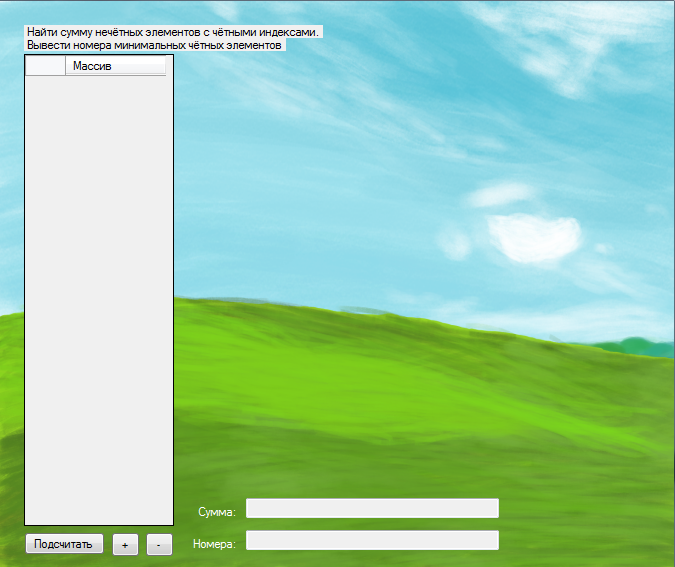
\includegraphics[width=0.5\linewidth]{images/handling-data-easy/form.png}
\caption{Форма окна для задания <<Простые вычисления>>}
\label{handling-data-easy-form}
\end{figure}

\subsection{Таблица с описанием элементов формы}
Все элементы формы были переименованы для большей читаемости. В таблице \ref{tab:handling-data-easy-form} представлены все изменения.

\begin{table}
\centering
\begin{tabular}{|m{0.3\textwidth}|m{0.3\textwidth}|m{0.3\textwidth}|}
\hline
\textbf{Описание элементов формы} & \textbf{Список изменённых атрибутов} & \textbf{Новое значение атрибута} \\
\hline
\hline
Окно формы & Text & Обработка табличных данных \\
Верхняя метка заголовка & Name & taskLabel \\
Нижняя метка заголовка & Name & taskLabel2 \\
Таблица & Name & arrayGridView \\
Кнопка <<Подсчитать>> & Name & countButton \\
Кнопка <<Добавить элемент>> & Name & addButton \\
Кнопка <<Удалить последний элемент>> & Name & popButton \\
Метка <<Сумма>> & Name & sumOddLabel \\
Метка <<Номера>> & Name & minsLabel \\
Поле для суммы & Name & outputOddSumTextBox \\
Поле для номеров & Name & outputMinsTextBox \\

\hline
\end{tabular}
\caption{Значение атрибутов элементов в приложении для обработки табличных данных}
\label{tab:handling-data-easy-form}
\end{table}

\subsection{Примеры правильной и неправильной работы приложения}
При запуске приложения на экране появляется окно \ref{fig:handling-data-easy-start}.

\begin{figure}
\centering
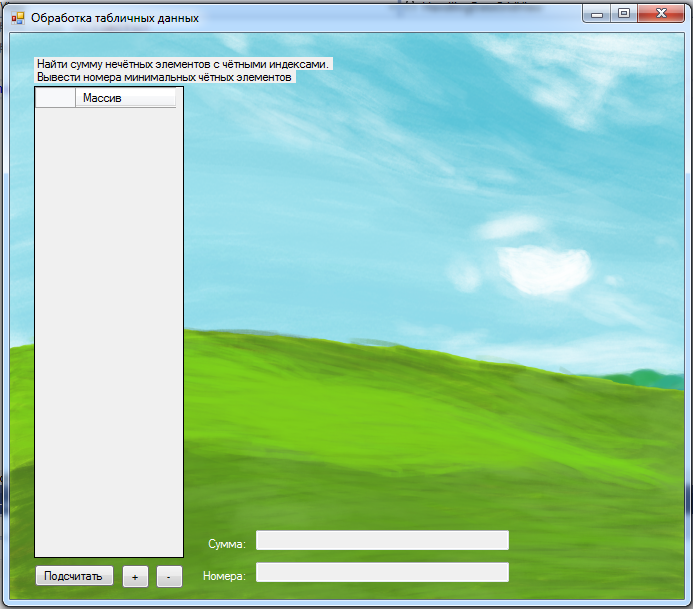
\includegraphics[width=0.5\linewidth]{images//handling-data-easy/start.png}
\caption{Запуск программы}
\label{fig:handling-data-easy-start}
\end{figure}

При нажатии на кнопку подсчитываются и подставляются значения в поля вывода. Также происходит обработка ошибок.

\begin{figure}
\centering
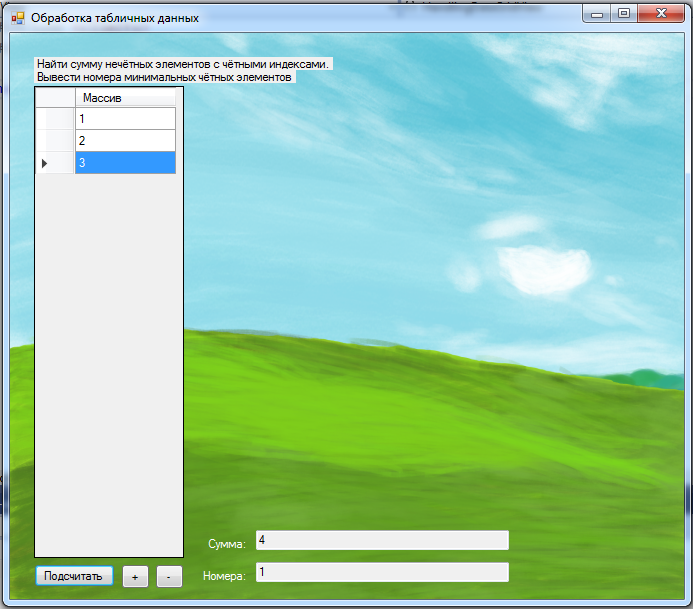
\includegraphics[width=0.5\linewidth]{images//handling-data-easy/okay.png}
\caption{Запуск с корректными данными}
\label{fig:handling-data-easy-okay}
\end{figure}

\begin{figure}
\centering
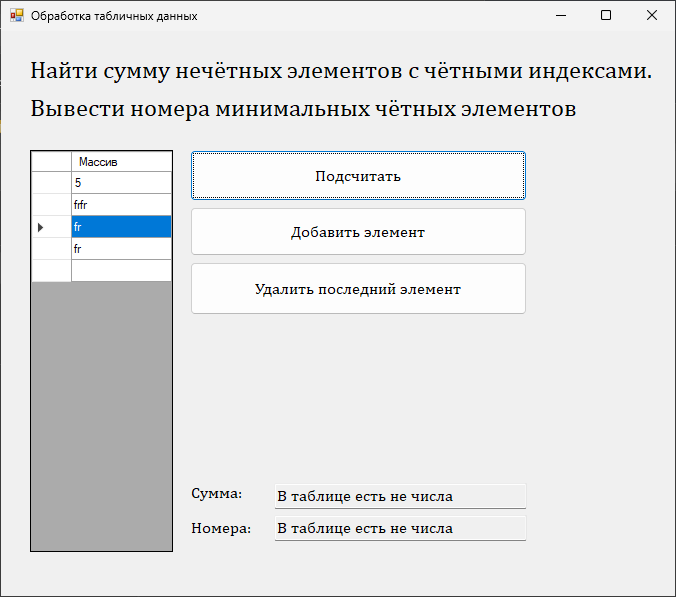
\includegraphics[width=0.5\linewidth]{images//handling-data-easy/error.png}
\caption{Пример ввода с некорректными данными}
\label{fig:handling-data-easy-error}
\end{figure}

\begin{figure}
\centering
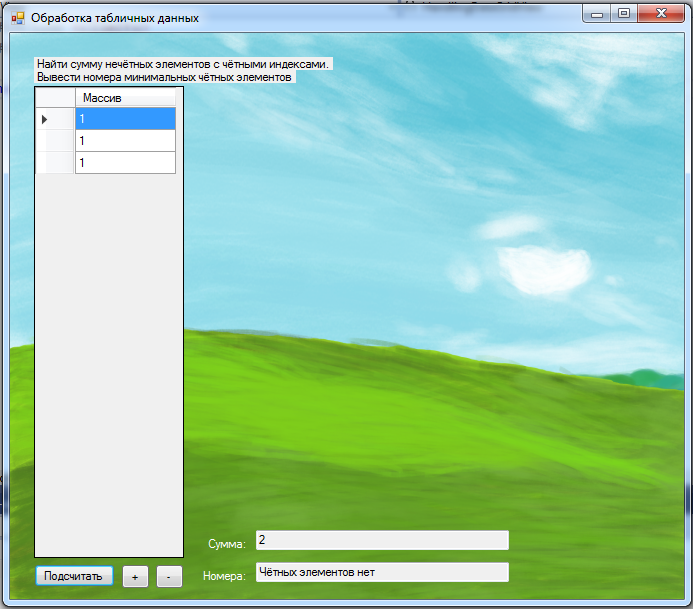
\includegraphics[width=0.5\linewidth]{images//handling-data-easy/error2.png}
\caption{Пример ввода с некорректными данными}
\label{fig:handling-data-easy-error2}
\end{figure}

\begin{figure}
\centering
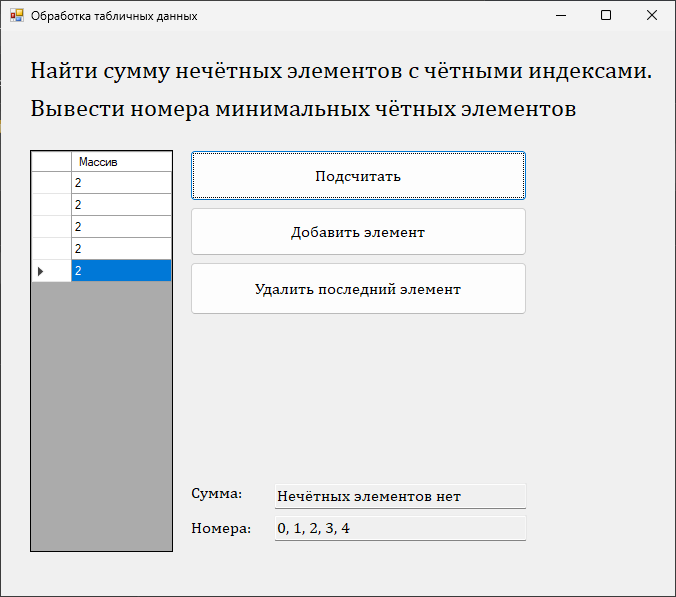
\includegraphics[width=0.5\linewidth]{images//handling-data-easy/error3.png}
\caption{Пример ввода с некорректными данными}
\label{fig:handling-data-easy-error3}
\end{figure}

\subsection{Примеры исходного кода}
\begin{minted}{cpp}
/* функция для обсчёта массива данных */
private: System::Void countArray(System::Object^ sender, System::EventArgs^ e) {
    long long sum = 0;
    long long minEl = LLONG_MAX;
    
    String^ columnName = "Массив";
    String^ resultSum;
    String^ resultIdx;

    // флаги для ошибок
    bool error = false;
    bool ifOdds = false;
    bool ifOddsOnEvenIdx = false;
    bool ifEvens = false;
    
    for (int i = 0; i < this->arrayGridView->RowCount; ++i) {
        long long val;
        Object^ cellValue = this->arrayGridView->Rows[i]->Cells[columnName]->Value;
    
        if (cellValue != nullptr) {
            try {
                val = Convert::ToInt64(cellValue);
                if (val % 2 != 0 && i % 2 == 0) {
                    sum += Convert::ToInt64(cellValue);
                    ifOddsOnEvenIdx = true;
                    ifOdds = true;
                }
                else if (val % 2 != 0) ifOdds = true;
                else {
                    ifEvens = true;
                    if (val < minEl) {
                        minEl = val;
                        resultIdx = Convert::ToString(i);
                    }
                    else if (val == minEl) {
                        resultIdx += ", " + Convert::ToString(i);
                    }
                }
            }
            catch (FormatException ^ e) {
                resultSum = "В таблице есть не числа";
                resultIdx = resultSum;
                error = true;
                break;
            }
        }
    }
    
    if (!error) resultSum = Convert::ToString(sum);
    if (!error && !ifOddsOnEvenIdx) resultSum = "Таких элементов нет";
    if (!error && !ifOdds) resultSum = "Нечётных элементов нет";
    
    if (!error && !ifEvens) resultIdx = "Чётных элементов нет";
    
    this->outputOddSumTextBox->Text = resultSum;
    this->outputMinsTextBox->Text = resultIdx;
}
\end{minted}

Больше кода проекта доступно в приложении \ref{application-A}. Также в приложенном архиве можно найти полный код проекта.